\documentclass[12pt]{article}
%Gummi|065|=)
\usepackage{amsmath, amsfonts, amssymb}
\usepackage[margin=0.5in]{geometry}
\usepackage{xcolor}
%\usepackage{graphicx}
%\usepackage{graphicx}
\newcommand{\off}[1]{}
\DeclareMathSizes{20}{30}{21}{18}

\newcommand{\myhrule}{}

\newcommand{\two }{\sqrt[3]{2}}
\newcommand{\four}{\sqrt[3]{4}}

\newcommand{\dash}{
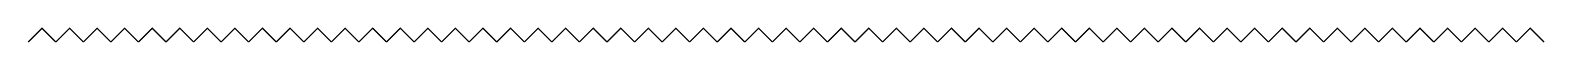
\begin{tikzpicture}[scale=0.35]
\foreach \x in {1,...,55}{
	\draw (\x,-0.25)--(\x+0.5,0.25)--(\x+1,-0.25);
}
\end{tikzpicture}
}

\newcommand{\sq}[3]{
\node at (#1+0.5,#2+0.5) {#3};
\draw (#1+0,#2+0)--(#1+1,#2+0)--(#1+1,#2+1)--(#1+0,#2+1)--cycle;
}

\usepackage{tikz}

\title{\textbf{ Circle Inversions: A Guide}}
\author{John D Mangual}
\date{}
\begin{document}

\fontfamily{qag}\selectfont \fontsize{25}{30}\selectfont

\maketitle

\noindent How does a circle map to another circle under the map $z \mapsto z + a$ and $z \mapsto - \frac{a}{z}$ ? 
$$ z \mapsto \frac{az+b}{cz+d}$$
Working our way up to the general transformation\footnote{To no avail, I have asked for explicit formulas for \textbf{inversions} - certain geometric transformations taking a circle to another circle.  And I get referred from one book to another.  And I will have to put together my own guide. }. \\ \\
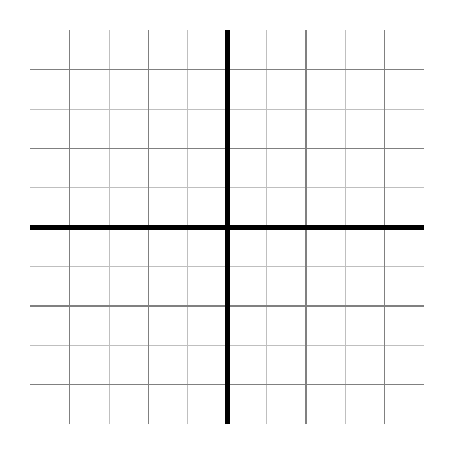
\begin{tikzpicture}
\foreach \a in {-2,-1.5,...,2} {
\draw[color=black!25!white] (-2.5,\a)--(2.5,\a);
\draw[color=black!25!white] (\a, -2.5)--(\a,2.5);
}
\foreach \a in {-2,-1,...,2} {
\draw[color=black!50!white] (-2.5,\a)--(2.5,\a);
\draw[color=black!50!white] (\a, -2.5)--(\a,2.5);
}
\draw[line width=2] (-2.5,0)--(2.5,0);
\draw[line width=2] (0,-2.5)--(0,2.5);
\end{tikzpicture} \\ \\
It doesn't make much sense to talk about theory.  I am trying to draw the image of circles under fractional linear transformation.

\newpage 
 
\noindent \textbf{Shifts} \\ \\
There are some cases that don't require a calculator. Such as $z \mapsto z + a$ and those maps are reasy to write down.

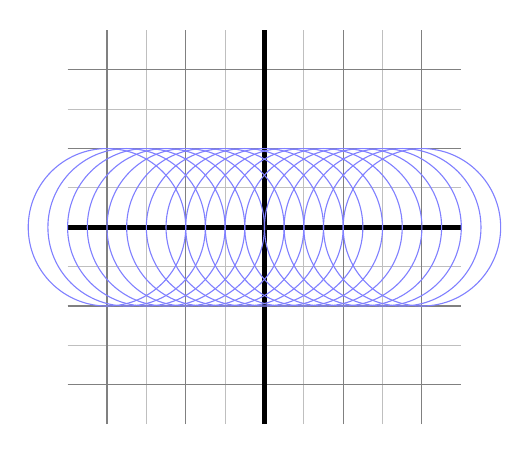
\begin{tikzpicture}
\foreach \a in {-2,-1.5,...,2} {
\draw[color=black!25!white] (-2.5,\a)--(2.5,\a);
\draw[color=black!25!white] (\a, -2.5)--(\a,2.5);
}
\foreach \a in {-2,-1,...,2} {
\draw[color=black!50!white] (-2.5,\a)--(2.5,\a);
\draw[color=black!50!white] (\a, -2.5)--(\a,2.5);
}
\draw[line width=2] (-2.5,0)--(2.5,0);
\draw[line width=2] (0,-2.5)--(0,2.5);

\foreach \a in {-2,-1.75,...,2} {
\draw[color=blue!50!white] (\a,0) circle (1);
}

\end{tikzpicture}  \\
here is variation where we change the formula:

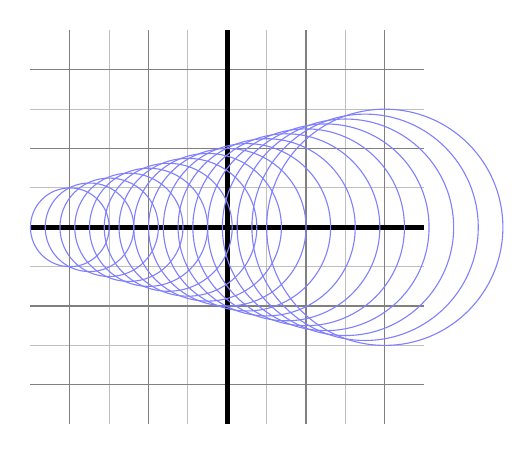
\begin{tikzpicture}
\foreach \a in {-2,-1.5,...,2} {
\draw[color=black!25!white] (-2.5,\a)--(2.5,\a);
\draw[color=black!25!white] (\a, -2.5)--(\a,2.5);
}
\foreach \a in {-2,-1,...,2} {
\draw[color=black!50!white] (-2.5,\a)--(2.5,\a);
\draw[color=black!50!white] (\a, -2.5)--(\a,2.5);
}
\draw[line width=2] (-2.5,0)--(2.5,0);
\draw[line width=2] (0,-2.5)--(0,2.5);

\foreach \a in {-2,-1.75,...,2} {
\draw[color=blue!50!white] (\a,0) circle ( 0.25*\a + 1  );
}
\end{tikzpicture} \\
The other formula is $z \mapsto -\frac{a}{z}$ that minus sign preserves the orientation of the complex plane (it looks identical). \\
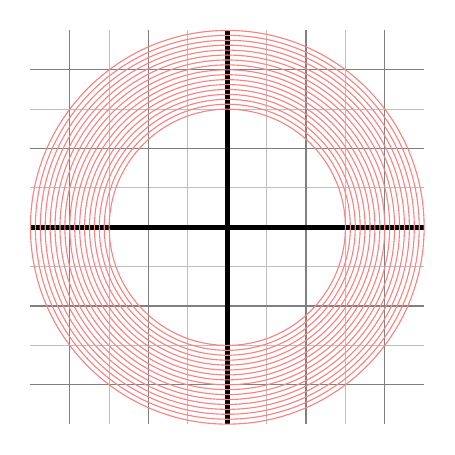
\begin{tikzpicture}
\foreach \a in {-2,-1.5,...,2} {
\draw[color=black!25!white] (-2.5,\a)--(2.5,\a);
\draw[color=black!25!white] (\a, -2.5)--(\a,2.5);
}
\foreach \a in {-2,-1,...,2} {
\draw[color=black!50!white] (-2.5,\a)--(2.5,\a);
\draw[color=black!50!white] (\a, -2.5)--(\a,2.5);
}
\draw[line width=2] (-2.5,0)--(2.5,0);
\draw[line width=2] (0,-2.5)--(0,2.5);

\foreach \a in {-2,-1.75,...,2} {
\draw[color=red!50!white] (0,0) circle (0.25*\a+2);
}

\end{tikzpicture}

\newpage

\fontfamily{qag}\selectfont \fontsize{12}{10}\selectfont


\begin{thebibliography}{}

\item Kurt Johansson \textbf{Discrete orthogonal polynomial ensembles and the Plancherel measure} \texttt{arXiv:math/9906120}

\item Graham Lagarias Mallows Wilks Yan \textbf{Apollonian Circle Packings: Geometry and Group Theory I. The Apollonian Group} \texttt{arXiv:math/0010298}

\item Caroline Series \textbf{The Modular Surface and Continued Fractions} \\ J. London Math. Soc. (1985) s2-31 (1): 69-80.
\texttt{doi: 10.1112/jlms/s2-31.1.69}




\end{thebibliography}



\end{document}